% Traduction française COMIMa de l'énoncé original (anglais).
$A$ annonce un chiffre, puis $B$ place ce chiffre dans l'une des cases vides, et ainsi de suite jusqu'à ce que les $8$ cases soient remplies. Chaque ligne forme un nombre de $4$ chiffres, et la différence considérée est le nombre de la ligne du haut moins celui de la ligne du bas. $A$ veut rendre cette différence la plus grande possible, $B$ la plus petite possible. Montrer que $B$ peut placer les chiffres de sorte que la différence soit au plus $4000$, et que $A$ peut annoncer les chiffres de sorte que la différence soit au moins $4000$.
\begin{center}
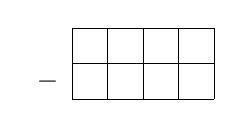
\begin{tikzpicture}[scale=0.45]
\draw (0,0) grid (4,2);
\node at (-0.7,0.5) {$-$};
\end{tikzpicture}
\end{center}
